\documentclass[12pt]{article}
\usepackage{pictex,amsmath,amssymb,amsbsy,amsfonts}
\usepackage{graphics,graphicx}
\usepackage{mathabx}

\setlength{\voffset}{-0.25in}
\setlength{\headsep}{+0.5in}
\setlength{\parskip}{1em}
\setlength{\parindent}{0em}

\def\vu{\mathbf{u}}
\def\vv{\mathbf{v}}
\def\vb{\mathbf{b}}
\def\vs{\mathbf{s}}
\def\vw{\mathbf{w}}

\usepackage{xcolor}
\usepackage{titlesec}
\usepackage{mdframed}
\usepackage[utf8]{vietnam}

\newmdenv[linecolor=blue,skipabove=\topsep,skipbelow=\topsep,leftmargin=5pt,rightmargin=-5pt,innerleftmargin=5pt,innerrightmargin=5pt]{mybox}

\begin{document}
\begin{center}
\textbf{DIGITAL SYSTEM}
\end{center}
\section{Digital and Analog Systems}
\begin{itemize}
	\item \textbf{Digital System} is a combination of devices that manipulate values represented in digital form.
	\item \textbf{Analog System} is a combination of devices that manipulate values represented in analog form.
\end{itemize}
\subsection*{Analog-to-digital conversion(ADC) and digital-to-analog conversion(DAC) complicate circuitry}
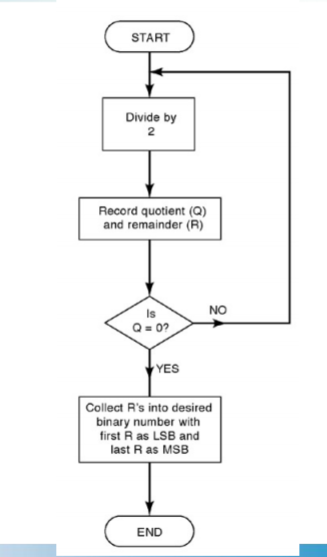
\includegraphics[scale=0.75]{hinh}
\section{Digital Number Systems}
-  Number system differ in the number of symbols they use\\
\begin{itemize}
	\item  Decimal - 10 symbols (base 10)
	\item  Hexadecimal - 16 symbols (base 16)
	\item  Octal - 8 symbols (base 8)
	\item  Binary - 2 symbols (base 2)
\end{itemize}
\section{Conversion}
\subsection*{Binary to Decimal Conversion}
1 \: 0 \: 0 \: 1 \: 0 \: $1_2$ \\
5 \: 4 \: 3 \: 2 \: 1  \:  0
We consider that:\\
$(100101)_2 = 1 \times 2^5 + 0 \times 2^4 + 0 \times 2^3 + 1 \times 2^2 + 0 \times 2^1 + 1 \times 2^0 = (37)_{10}$
\subsection*{Decimal to Binary Conversion}
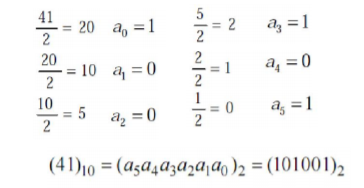
\includegraphics{hinh2}\\
\textbf{Flow chart:}\\
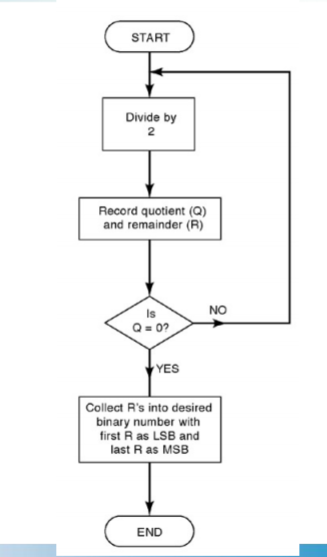
\includegraphics{hinh}
\subsection*{Convert from Hexadecimal to Decimal}
- Convert from Hexadecimal to decimal by multiplying each hex digit by its positional weight\\
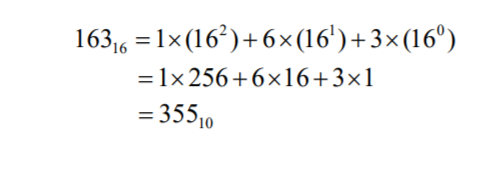
\includegraphics{hinh3}
\subsection*{Hexadecimal to Decimal Conversion}
- Convert form Hexadecimal to Decimal by deviding the decimal number by 16\\
Same method to convertion from binary to decimal\\
\subsection*{Hexadecimal to Binary Conversion}
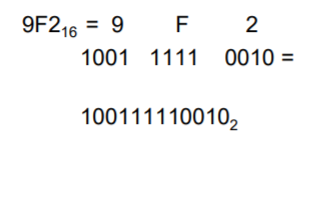
\includegraphics{hinh4}
\subsection*{Binary to Hexadecimal Convertion}
- To convert Binary to Hexadecimal, first we should group bits in four, then we convert each group to hexadecimal.\\
Ex:\\
$1110100110_2 = 0011 \: 1010 \: 0110$ \\
 = 3 \: A \: 6 \\
 = $3A6_{16}$
\section{BCD}
\begin{itemize}
	\item \textbf{Binary Coded Decimal} (BCD) is a another way to present decimal numbers in binary form.
 	\item BCD is widely uses and combines features of both decimal and binary systems.
 	\item Each digit is converted to a binary equivalent.
\begin{table}[h!]
\begin{center}
	\caption{BCD Table}
	\begin{tabular}{|c|c|}
	\hline
	\textbf{Decimal} & \textbf{BCD} \\
	\hline
	0 & 0000\\
	\hline
	1 & 0001\\
	\hline
	2 & 0010\\
	\hline
	3 & 0011\\
	\hline
	4 & 0100\\
	\hline
	5 & 0101\\
	\hline
	6 & 0110\\
	\hline
	7 & 0111\\
	\hline
	8 & 1000\\
	\hline
	9 & 1001\\
	\hline
	\end{tabular}
\end{center}
\end{table}
	\item To convert the number $874_{10}$ to BCD: \\
	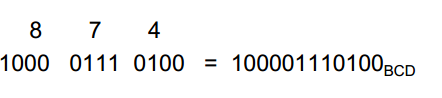
\includegraphics{hinh5}
	\item Each decimal digit is represented using 4 bits
	\item Each 4-bit group can never be greater than 9.
	\item Reverse the process to convert BCD to decimal.
\end{itemize}
\section{Flip Flop}
- So far we has seen Combinational Logic that the output(s) depends only on the value of the input variables. \\
- Here we look at Sequential Logic circuit that the output(s) can depend on present and also past values of the input and output variables. \\
- Sequential circuits exist only in one of a defined number of state at any one time.
\subsection{Synchronous and Asynchronous Sequence Logic:}
\begin{itemize}
	\item Synchronous: \\
	- The timing of all state transitions is controlled by a common clock. \\
	- Changes in all variables occur simultaneously.
	\item Asynchronous: \\
	- State transistions occur independently of any clock and normally dependent on the timing of transitions in the input variables. \\
	- Changes in more than one output do not neccessarily occur simultaneously.
	\item Clock:\\
	- A clock signal is a square wave of fixed frequency. \\
	- Often, transitions will occur on one of the clock pulses 
\end{itemize}
\subsection{General Flip Flop Symbol and definition of its two possible output states}
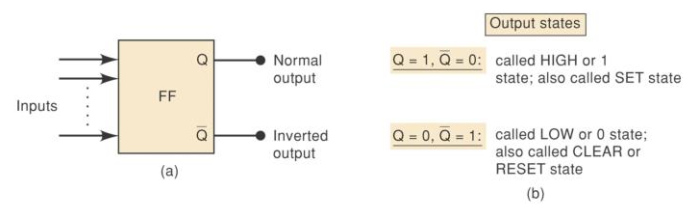
\includegraphics[scale = 0.75]{hinh6} \\
- The Flip Flop, abbreviated FF, is a key memory element.\\
- The output of the Flip Flop is Q and $\bar{Q}$. \\
- Q is understood to be the normal output, $\bar{Q}$ is always the opposite
- The most basic circuit can be constructed from either two NAND gates or NOR gates. The NAND gates version is called a \textbf{NAND gate latch}
\subsection{NAND gate latch}
- The inputs are \textbf{set} and \textbf{clear} (reset). \\
- The inputs are active low, that is, the output will change when the input is pulsed low. \\
- When the latch is set: 
\begin{center}
Q = 1 and $\bar{Q}$ = 0
\end{center}
- When the latch is clear or reset: 
\begin{center}
Q = 0 and $\bar{Q}$ = 1
\end{center}
\textbf{Summary of NAND latch} \\
\begin{itemize}
	\item SET = RESET = 1: Normal resting state, outputs remain in state prior to output.
	\item  SET = 0, RESET = 1: Q will go high and remain high even if the SET input goes high.
	\item SET = 1, RESET = 0: Q will go low and remain low even if the SET input goes high. 
	\item SET = RESET = 0: Output is unpredictable because the latch is being set and reset at the same time.
\end{itemize}
\subsection{NOR Gate Latch}
- The NOR Gate Latch is similar to the NAND Gate Latch, except that the output Q and $\bar{Q}$ is reserved. \\
- \textbf{The inputs are active high}, that is, the outputs will change only the inputs \textbf{are pulsed high}. \\
- In order to ensure that a FF begins operation at a known level, a pulse may be applied to SET and RESET inputs when a device is powered up.
\subsection{Digital Pulses}
- In digital system, when a signal switches from a normal inactive state to the oposite (active) state, thus causing something happen in the circuit. Then the signal returns to its inactive state while the effect of the recently activated signal remains in the system. These signals are called pulses.\\
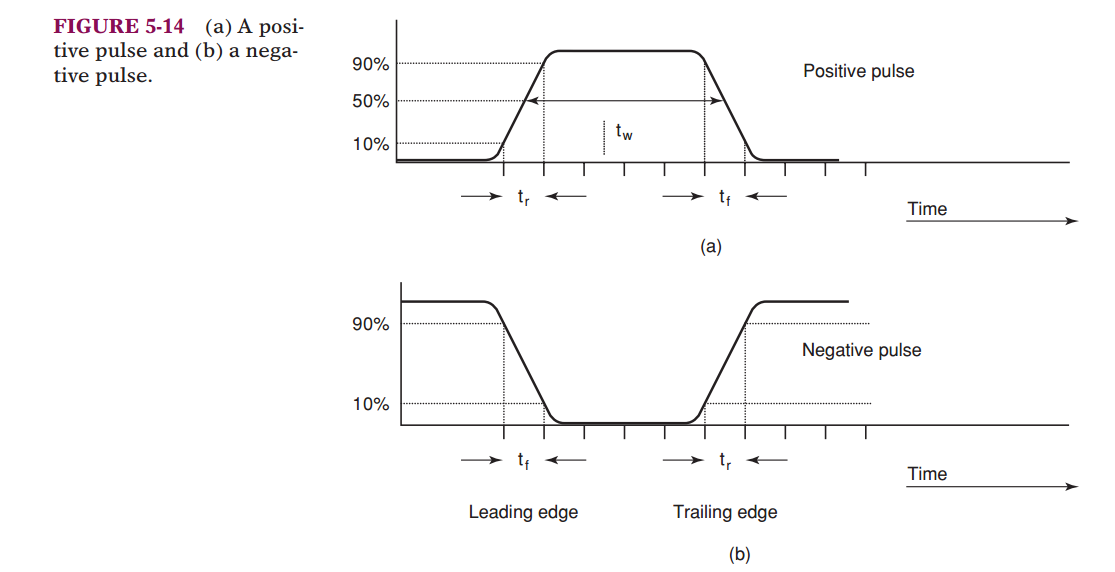
\includegraphics[scale=0.7]{hinh7}
\bigbreak
- A pulse that performs its intended function when it goes HIGH is called a positive pulse. \\
- A pulse that performs its intended funtion when it goes LOW is called a negative pulse. \\
- The transition from low to high on a positive pulse is called rise time ($t_r$). \\
- The transition from high to low on a positive pulse is called fall time ($t_f$). \\
- The transition from the beginning of the pulse is called the leading edge and the transition at the end of the pulse is called the trailing edge. \\
\subsection{Clock Signal and CLocked Flip Flop}
- Digital system can be operate either asynchronously and synchoronously:
\begin{itemize}
	\item In asynchronous system, the outputs of circuits can change state anytime one or more of the inputs change.
	\item In synchronous system, the outputs can change states at the exact time by a signal called clock. This clock signal is generally a rectangular pulse train or a square wave.
\end{itemize}
\textbf{Clock Signal}\\
- Most (if not all) of the system  outputs can change state only when the clock make a transition. \\
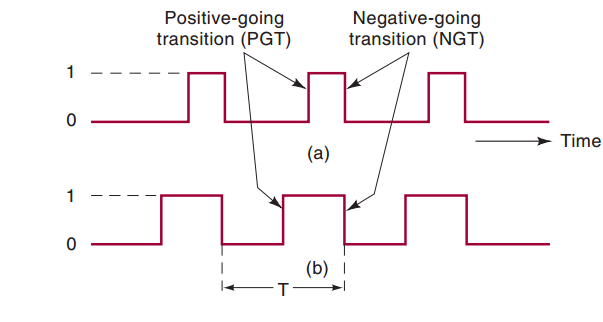
\includegraphics[scale = 0.7]{hinh8}
- A transition (also called \textit{edges}):
\begin{itemize}
	\item When the clock changes from 0 to 1, this is called the \textbf{positive-going transition (PGT)}.
	\item When the clock changes from 1 to 0, this called the \textbf{negative-going transition (NGT)}.
\end{itemize}
- Most digital system are pricipally synchronous (although there are always some asynchronous parts) because synchronous circuits are easier to design and troubleshoot.
\bigbreak
\textbf{Clocked Flip Flop} \\
\begin{itemize}
	\item CLocked FFs can change state on one or other clock transitions. Some common characteristics: \\
	- CLock inputs are labeled as CLK, CK, or CP.\\
	- A \textbf{small triangle} at the CLK input indicates that CLK input is activated with a PGT (positive-going transition). \\
	- A \textbf{bubble and a triangle} at the CLK input indicates that CLK input is activated with a NGT (negative-going transition). \\
	- Control inputs have an effect on the output only at the active clock transition (PGT and NGT). There are also called synchronous control inputs. \\
	- The control inputs get the FF outputs ready to change, but the change is not triggered until the CLK edge.
\end{itemize}
\bigbreak
\textbf{Setup Time and Hold Time} \\
- Setup time ($t_s$) is the minimum time interval before the active CLK transition that the control input must be kept at the proper level. \\
- Hold time ($t_h$) is the time after the active CLK transition during which the control input must be kept at the proper level.
\subsection{Clocked S-R Flip Flop}
- In Clocked S-R Flip Flop system, FF only change states when when a signal applied to its clock input makes a transition from 0 to 1 or from 1 to 0 (PGT and NGT). \\
- The up arrow ($\uparrow$) indicates that a PGT is required at CLK; the label $Q_{0}$ indicates the level at Q prior to the PGT. \\
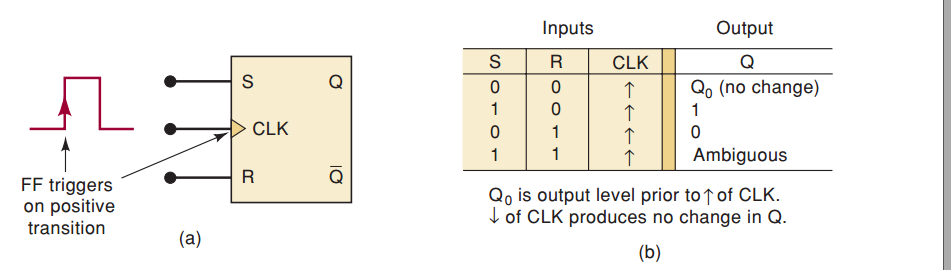
\includegraphics[scale = 0.7]{hinh10}
\bigbreak
- We can analyze these waveforms as follows: \\
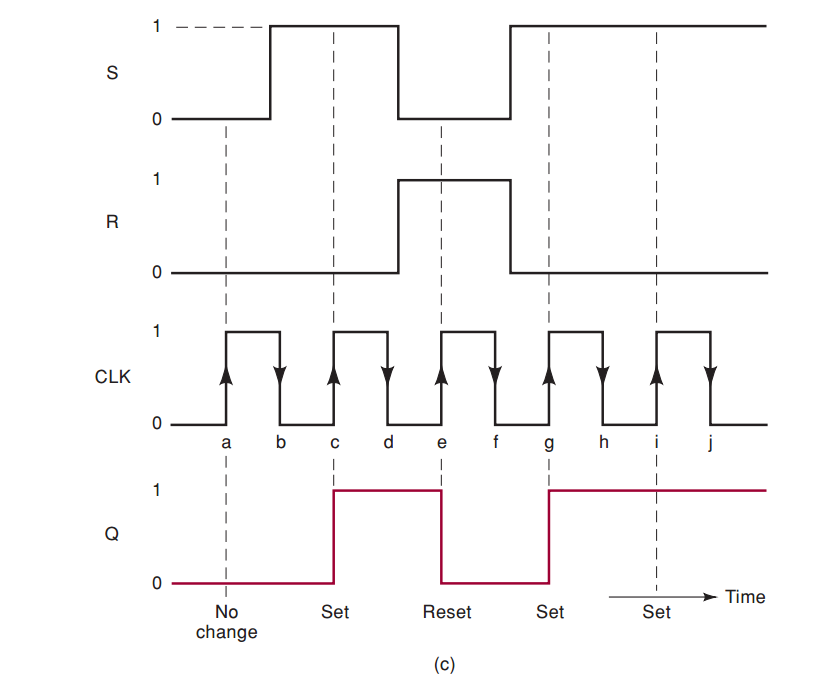
\includegraphics[scale = 0.7]{hinh9}
\bigbreak
\begin{enumerate}
	%1
	\item Initiallly all inputs are 0 and the Q output is assumed to be 0; that is $Q_0$ = 0
	%2
	\item When the PGT of the first clock pulse occurs (point a), the S and R inputs are both 0, so the FF is not effected and remains in the Q = 0 state (Q = $Q_0$)
	%3
	\item When the PGT of the second clock pulse (point c), the S = 1 and R = 0. Thus the FF set to 1 state at the rising edge of this clock pulse.
	%4
	\item When the third clock pulse makes its positive transition (point e) S = 0 and R = 1. Thus it causes the FF set to 0 state.
	%5
	\item At the fourh pulse set the FF once again to the Q = 1 state (point g) because S = 1 and R = 0 when PGT occurs
	%6
	\item The fifth pulse also find that S = 1 and R = 0 at PGT occurs so the FF remains state.
	%7
	\item The case that S = R = 1 should not be used because it results in an ambiguous condition.
	%8 
	\item It should be noted that those waveforms that the FF is \textbf{not effected} by the NGT of the clock pulses. Also note that the S and R levels have no effects on the FF, except upon the occurence of the PGT \textbf{in PGT transitions}
	%9
	\item For the NGT transition the FF operate at the same manner at PGT transition, except the output can change states only on the falling edge of the clock pulse 
\end{enumerate}
- As a general rule for stable flip flop triggering, the clock pulse rise and fall time must be very short, around typically 2 - 5 ns. \\
\subsection{Clocked J-K Flip Flop}
- The J and K inputs control the state of the FF in the same way as the S and R inputs do for the clocked S-R flip flop, except 1 difference that when J = K = 1 condition \textbf{does not result} in ambiguous output. In this condition, the FF will always go to its opposite side of the clock signal, this is called \textbf{toggle mode} of the operation.\\
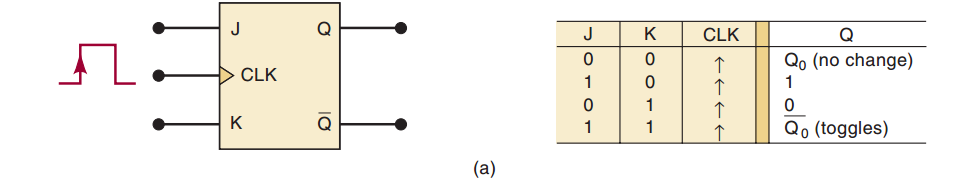
\includegraphics[scale = 0.8]{hinh11}
\bigbreak
- The operation of the J-K Clocked Flip Flop is the same as the S-R Clocked Flip Flop , except when J = K = 1 at the PGT transition the output will change to the opposite state. \\
- Also in NGT, the operation is still same as PGT when clock is triggered in NGT.\\
- In edge-triggered J-K Flip Flop, CLK* must be high for FF to change states. This condition only occurs at the edge of a CLK transition
\subsection{Clocked D Flip FLop}
- Unlike the S-R and J-K Clocked FLip Flop, this flip flop has only one synchronous control input, \textit{D}, which stands for data. \\
- The operation of the D  CLocked Flip Flop is very simple: Q will go as the same state on the D input when a PGT occurs at CLK. \\
- A negative-edge-triggered D flip flop operates in the same way and Q will take on the value of D when a NGT occurs at CLK. \\
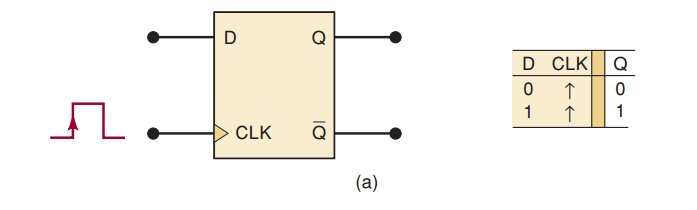
\includegraphics[scale=0.8]{hinh12}
\subsection{D Latch (Transparent Latch)}
-  The edge trigggered D Flip Flop uses an edge-detector circuit to ensure that the output will repond to the D input only when the active transition of the clock occurs. The latch that its edge-detector is not used called the D latch.
\begin{itemize}
	\item One data input.
	\item The clock has been replaced by an ENABLE (EN).
	\item The device is not edge-triggered.
	\item When EN = 1; the output follows the change of input.
	\item When EN = 0; wheither D changes or not Q will stay at their current level (no change).
\end{itemize}
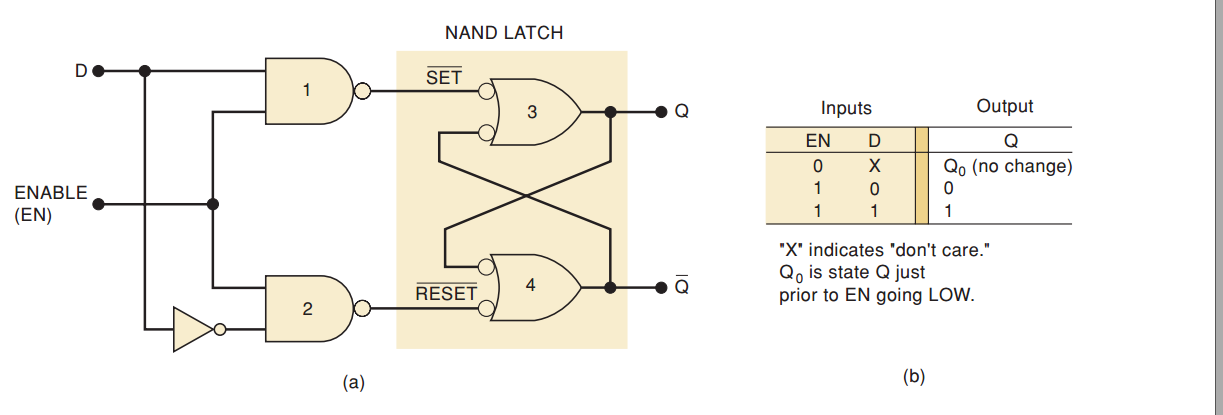
\includegraphics[scale = 0.8]{hinh13}
\bigbreak
- Logic symbol of D latch: \\
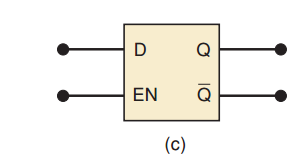
\includegraphics[scale = 0.85]{hinh14}
\subsection{Asynchronous Inputs}
\begin{itemize}
	\item For the clocked flip flop, the S-R, J-K and D inputs have been reffered as \textbf{synchronous inputs} 
	\item Most clocked FF also have one or more asynchronous inputs that operate independently of the synchronous inputs. 
	\item These asynchronous inputs can be used to set FF to the 1 state of clear (reset) and FF to 0 state at \textbf{any time, regardless conditions of inputs}.
	\item State in another way, the asynchronous inputs are \textbf{overide inputs}
\end{itemize}
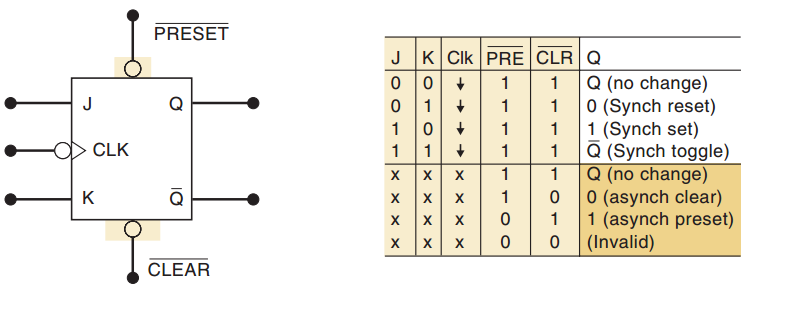
\includegraphics[scale = 0.85]{hinh15.png}
\bigbreak
- $\overline{PRESET} = \overline{CLEAR} = 1$: The asynchronous inputs are inactive and the output depend only on CLK transitions. \\
- $\overline{PRESET} = 0; \overline{CLEAR} = 1$: The $\overline{PRESET}$ is activated and Q = 1 (no matter what conditions). The CLK inputs cannot affect the FF while $\overline{PRESET}$ = 0. \\
- $\overline{PRESET} = 1; \overline{CLEAR} = 0$: The $\overline{CLEAR}$ is activated and Q = 0 (no matter what conditions). The CLK inputs cannot affect the FF while $\overline{CLEAR}$ = 0. \\
- $\overline{PRESET} = \overline{CLEAR} = 0$: Ambiguous response. \\ 
\end{document}